\Chapter{}{East Asian Dust}\label{chap:east_asia_dust}
The previous chapter described the important role of dust in the climate system and the physical processes included in current dust models. This chapter will narrow down the scope and bring the \acrshort{clp} in focus. 
The first section will describe spatial distribution and characteristics of the dust sources in East Asia. 
Then in the second section will introduce the \acrshort{clp} and examine how dust deposited over the \acrshort{clp} can be traced back to the source regions. 
The two last sections of this chapter will look into what kind of weather that produces dust storms in the region and the climatic factors that decides the frequency of dust storms.    
% East Asian region has a long-lasting history of aeolian processes and much of this history is recorded in the \acrshort{clp}. 
% In the second and last part of this chapter, the scope is narrowed down to the East Asian region. It will begin by describing the location and characteristics of the main source and dust fallout regions, followed by an overview of the meteorological conditions responsible for producing dust events and their climatology. 
% The East Asian region has a long-lasting history of aridity. The oldest evidence of aridification in this region dates back to the late Oligocene \parencite{qiang2011new}. Since the Miocene, global cooling and combined with the uplift of the Tibetan Plateau have further expanded the arid environment of Northern East Asia \parencite{miao2012controlled}.  
% The focus of this thesis is the East Asian dust sources and how the dust gets transported and deposited over the \acrshort{clp}. Conversely, this section will introduce the study area and describe the spatial and temporal variations of dust emissions in this region.  

\section{Spatial distribution and characteristics of dust sources}\label{sec:spatial_temporal_dust}
\begin{figure}
    \centering
    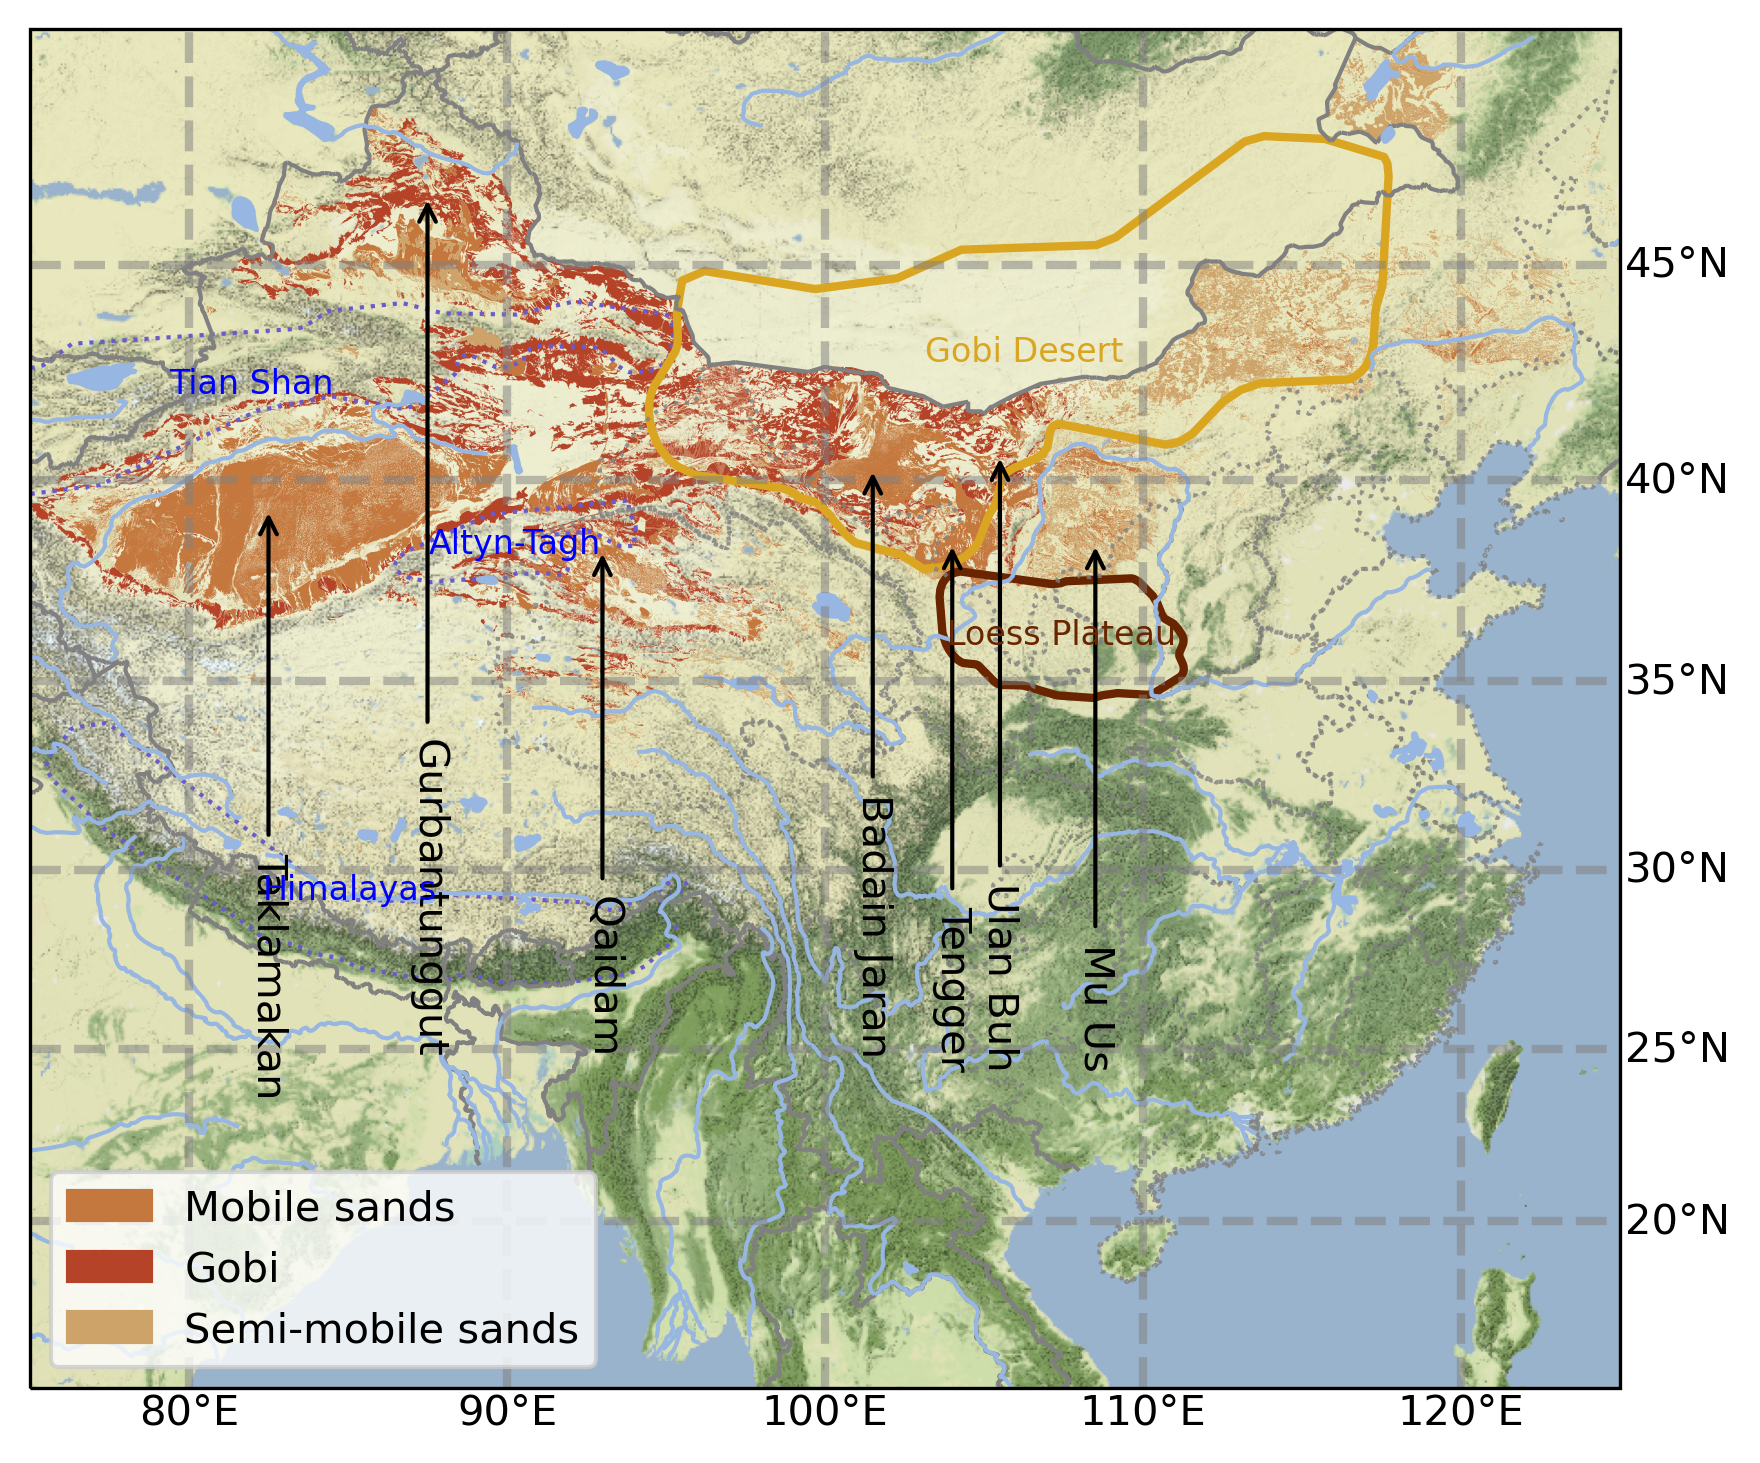
\includegraphics[width=0.9\textwidth]{texfiles/figs/map_sources_china.png}
    \caption{The major deserts in East Asia, with the mobile sands, semi-mobile sands and Gobi regions areas indicated, modified from \textcite{mao2013numerical}. }
    \label{fig:maps_deserts}
\end{figure}
The majority of the East Asian deserts are located in the Northern part of China and South East Mongolia, as shown in \Cref{fig:maps_deserts}. The precipitation patterns predominately determine the distribution of the deserts.
Situated in the interior of the Eurasian continent, the deserts are far removed from the moisture of the Pacific Ocean. 
The dry conditions are exacerbated by the Tibetan Plateau and the Himalayas, inhibiting the transport of moist air masses from the southwest.  
In total, the East Asian deserts make up the second-largest source of atmospheric dust on the planet with an approximate annual dust emissions of 2000 Mt \parencite{chen2017overview}. 

In terms of the morphology and composition of the surface soil, the East Asian deserts can be separated into two classes gobi-deserts and sand deserts \parencite{xuan2002characterization}. The Gobi is characterised by regions consisting of pebbles, gravel and rock debris. Accordingly, the Gobi desert refers to an area consisting of interluding regions of sandy deserts, gobies and grasslands.
Gobies and the Gobi desert mainly cover the northern region of the Inner Mongolia Plateau and the southern part of Mongolia (\Cref{fig:maps_deserts}b). \todo{add some more info on Gobi}

The interior of East Asia also fosters many sand deserts that mainly consists of loose sand. 
The loose sand facilitates dune formation, and the worlds tallest dunes are situated in the Badain Jaran desert. 
The Badain Jaran desert has dunes so large that they can generate their own weather \parencite{dong2013investigation}. 
The most significant sand desert in the region is the Taklamakan desert, located in the Tarim Basin. 
The Tarim Basin is extremely dry, with annual precipitation of as low as 20mm \parencite{shao2006review}. 
The extreme dryness makes it impossible for vegetation to set root, conversely the region has a very small threshold friction velocity of about 4 m/s compared to 7 m/s for the Gobi desert \parencite{ShaoYaping2008PaMo}. 
Therefore, the Taklamakan experience the highest number of days with blowing sand among the East Asian deserts.
However, the desert is well shielded from the weather by tall 3000 meters mountain ranges (Tian Shan to the north, Pamir plateau to the west and Kunlun Mountains to the south) on all sides except for the opening at the eastern side of the basin. 
Therefore severe dust storms forms less frequently in Taklamakan \parencite{ShaoYaping2008PaMo}. 

There are also several deserts located in close proximity of \acrshort{clp}. Among the larger deserts being the Tegger desert, Ulan Buh desert and Mu Us desert. \todo{some more about the near clp desert?}

\section{The Chinese Loess Plateau}
\begin{figure}[htpb]

        \centering
        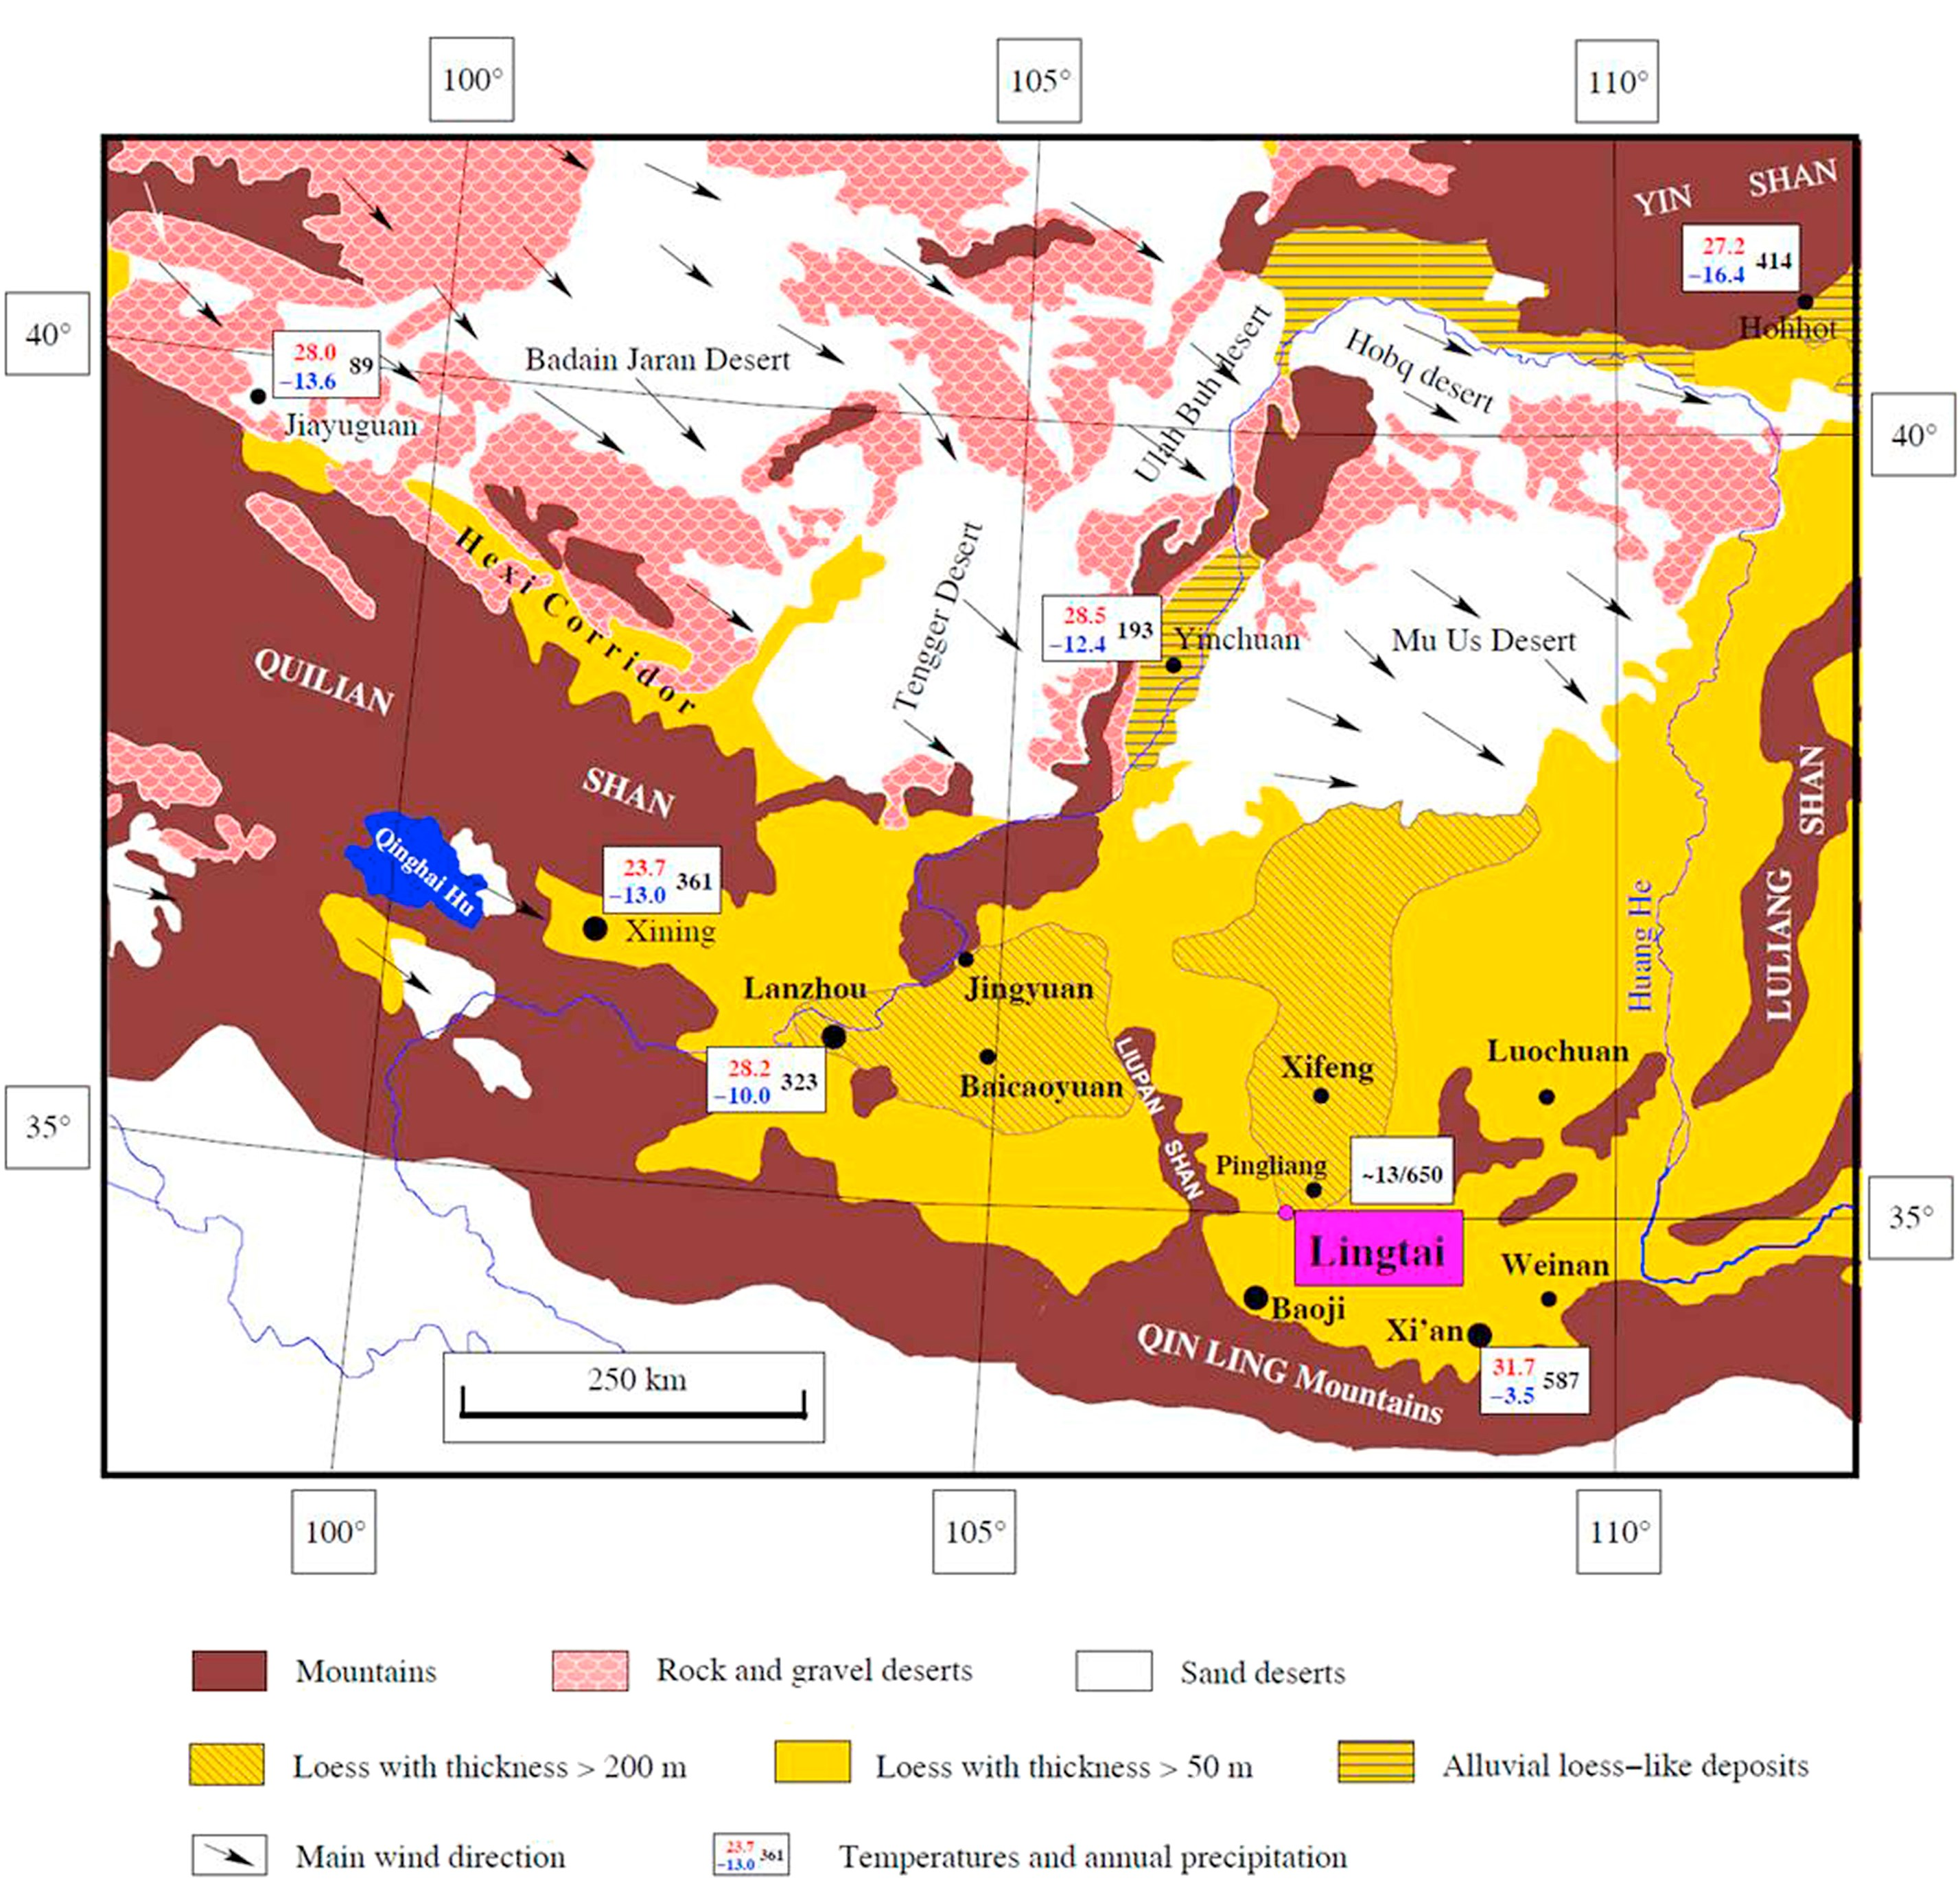
\includegraphics[width=0.85\textwidth]{texfiles/figs/loess_plateau_maps.jpg}
        

    \caption{Map of the \acrshort{clp}, adopted from \textcite{spassov2002loess}.}
    \label{fig:map_clp}
\end{figure}

A large portion of the dust emitted from the desert regions in East Asia gets transported and deposited over the \acrshort{clp}. 
The \acrshort{clp} covers an area of around \SI{450000}{\square\km}. In some places the thickness of the loess deposits are excess of 200m e.g. Lanzhou (see \Cref{fig:map_clp}). 
The total volume of deposited dust contained at the \acrshort{clp} is huge, approximately 0.2 million \si{\cubic\km}, equivalent to the volume of the Scandinavian mountains \parencite{maher2016palaeoclimatic}.  
The Chinese loess record consists of two main sequences, the Quaternary and the Red Clay sequence. The Quaternary sequence consists of alternating layers of paleosols and loess that spans the entire Quaternary extending into the Pleistocene \parencite{maher2016palaeoclimatic}. 
The alternating paleosol and loess layers indicate the inter-glacial and glacial periods.  Underlying the Quaternary sequence is the Red Clay sequence which is of similar aeolian origin and extend the loess record into the Miocene. 
In contrast to the Quaternary sequence, the Red Clay sequences are continuous without interluding paleosol layers. Suggesting that the Red Clay was formed under relative humid conditions in contrast to the colder climate during the Quaternary glacial periods \parencite{yang2004comparison}. 

Both sequences are well sorted and mostly composed of silt-sized particles between 3 and \SI{40}{\micro\metre} with a modal grain size that varies between 4 and \SI{8}{\micro\metre} \parencite{maher2016palaeoclimatic}.
In terms of the spatial variation across the \acrshort{clp} the mode of the of the grain size distribution typically becomes coarser along the transect from south east to north west of the plateau \parencite{ding2000re}. 
Moreover the loess \acrfull{mar} and thickness is the highest in the northern and western part of the plateau \parencite{maher2016palaeoclimatic}.    

The spatial variation in the provenance of the \acrshort{clp} loess has been investigated both for the  Red Clay  \parencite{shang2016variations} and Quaternary sequence \parencite{bird2015quaternary}. 
% and present day \parencite{sun2003seasonal}. 
\textcite{shang2016variations} investigated the spatial variation in the provenance of the Red Clay, where they found that the southern \acrshort{clp}  (Lingtai, Lantian and Luochuan) had U-Pb age distributions similar to that of the northern Tibetan Plateau and Taklamakan compared to eastern \acrshort{clp} (Baode) which in addition had a peak at 200-300 similar to the age distribution of the Mu Us desert. 
Regarding the Quaternary sequence, \textcite{bird2015quaternary} found using same U-Pb dating technique as \textcite{shang2016variations} that the \acrshort{clp} deposits primarily shared age signatures with the northeastern \acrfull{tp} and Qaidam Basin.
However, they also found distinct spatial variability among the sites with the northeastern \acrshort{clp} receiving a larger contribution from the northern deserts.   
The challenge of determining the provenance of the loess is that the assumed source should reasonably account for all the features of the loess and not just some of the loess characteristics \parencite{maher2016palaeoclimatic}.

\textcite{sun2003seasonal} investigated the spatial and seasonal variability of modern dust deposition over the \acrshort{clp} along a south north transect across the \acrshort{clp}. 
The seasonal variability in the \acrshort{mar} of modern dust, showed highest values in spring and lowest values in autumn and winter at all sites the along the transect, but the amplitude in seasonal variability of the \acrshort{mar} was greatest at the northern most site. The mode of the 
\section{Meteorological conditions of dust storms}

In East Asia about 80\% of the dust events occurs in spring months from March until May, with half of the dust events occurring in April \parencite{sun2001spatial}. 
The occurrence of dust events are strongly correlated with the surface wind speed \parencite{kurosaki2003recent}. 
Strong surface wind speeds are typically generated by passing cold fronts and synoptic scale cyclones associated with cold air outbreaks \parencite{sun2001spatial, zhou2003typical, takemi2005dust}.
Moreover cold fronts promotes strong and deep vertical mixing due to the strong surface heat flux in the cold frontal region. The deep mixed layer can carry the dust into the upper troposphere allowing the dust to be transported far downwind \parencite{liu2003high}. 
  
Dust storms in Gobi desert and the desert regions north west of the \acrshort{clp} are usually due to the development of cyclones over Mongolia \parencite{shao2006review}. 
The dust storm forms within the frontal region of the cyclone to the south east of the central low pressure \parencite{takemi2005dust}. 
The cold air outbreaks that produces dust event in this region typically follow a northerly path, passing near lake Baikal and the moving southward across across southern Mongolia and China \parencite{sun2001spatial}. 

Whereas dust storms in the Gobi and north western deserts are a direct consequence of synoptic scale circulation, Taklamakan is less influenced by the large scale circulation due to its shielded location in the Tarim Basin \parencite{takemi2005dust}.
Rather cold air intrusions caused by the synoptic conditions is the predominate cause of dust storm in Taklamakan. 
\textcite{aoki2005dust} identified three primary patterns of dust storm genesis in the Taklamakan desert. 
The first pattern is characterised by a cold pool located to the north of the Tian Shan creating a strong temperature gradient between the cold pool and the inside of the the basin. 
The cold air forms a gravity current that intrudes into the basin from the east, producing strong surface winds. 
The strong winds initiated the dust storm in the eastern end of the basin and then moves westward until eventually the whole basin is enveloped. 
The second pattern is characterised by northerly flow with a trough located on the northern side of the Tian Shan. 
As the though advances the accompanying cold pool moves over the Tian Shan rather than around, directly into the basin, with similar flow characteristics as the first pattern except for the wind direction. 
These dust storms occur over a broad area of the desert. In contrast to the first two patterns the third pattern primarily produces dust storm in the western part of the desert. This pattern occur when the 500hPa trough advances eastward passing over the Parmir plateau bringing along cold air that flows into basin along the western slope. 
%However not all dust storms in the Tarim basin are the consequence of synoptic scale disturbances dust storms can also be           

In the recent decades there have been observed a large decrease in the number of dust  
which has been hypothesised to be a consequence of arctic amplification resulting in a weakened temperature gradient \parencite{liu2020impact}.

%The number of cold air outbreaks occurring in spring is much influenced by the intensity and location of the jet stream. A strong jet stream inhibits air mass exchange between lower and higher latitudes whereas and confine the cold air to the high latitudes \parencite{wang2008variability}. There has been a large decrease in the number of dust events in East Asia since the 1980s, which has been hypothesised to be the result of arctic amplification and weakened temperature gradients \parencite{liu2020impact}. 

\section{Influence of regional and large-scale climatic factors on dust storms}
\begin{figure}[htpb]
    \centering
    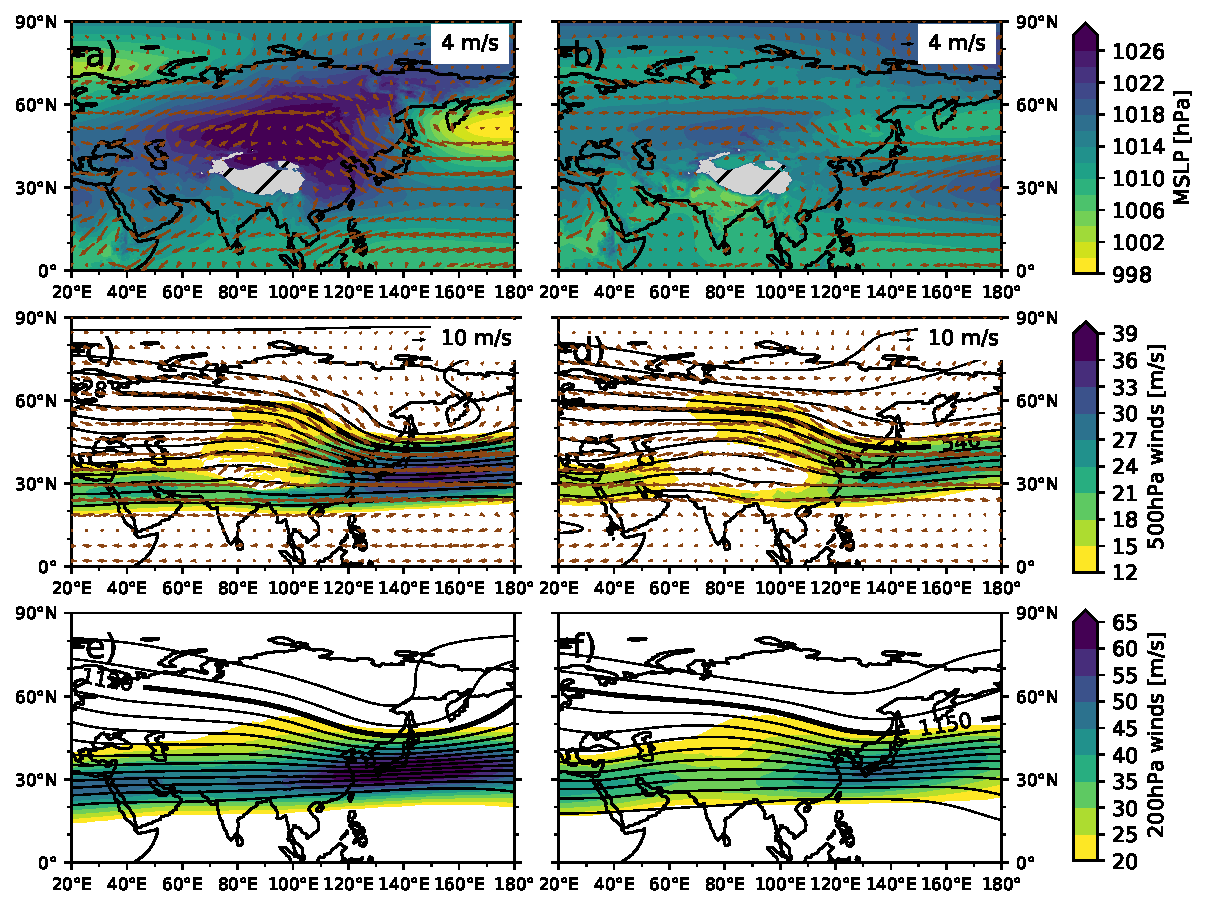
\includegraphics[width=\textwidth]{texfiles/figs/climatology_1999-2019.pdf}
    \caption{The 20 year average of winter (DJF)  and spring (MAM) circulation from ERA5. (a) Winter and (b) spring \acrshort{mslp} and 850hPa winds climatology. (c) Winter and (b) spring 500hPa geopotential height and winds. (e) winter and (f) spring 200hPa geopotential height and wind speed.}
    \label{fig:clim_circulation}
\end{figure}

Even though dust storms are primarily a spring phenomena, the conditions of the preceding winter have been shown to have a significant influence on the spring dust storm frequency \parencite{he2017impact, liu2018influence, gong2006simulated}. The East Asian winter climate is dominated by the \acrfull{eawm}. 
The \acrshort{eawm} is driven by the temperature contrast between the relatively cold Eurasian continent and North Pacific Ocean.
The \acrshort{tp} also plays an important role in the \acrshort{eawm}. First and foremost the high altitude and excessive snow cover of the \acrshort{tp} amplifies the land-sea temperature contrast, and second the topography forces the subtropical westerly jet to follow along the southerly margins of the Himalayas \parencite{tada2016evolution}. 
The characteristic features of the \acrshort{eawm} are the \acrfull{sh}, \acrfull{al}, low-level north easterlies, mid-level \acrfull{eat}, and the high-level East Asian jet stream. 
\Cref{fig:clim_circulation} shows the climatology of the winter and spring  circulation. 
In winter the \acrshort{sh} is distinct. 
The strength of the \acrshort{sh} is a deciding factor for the frequency of dust storms due to how the \acrshort{sh} regulates the occurrences of cold air outbreaks.
% occur when the pressure of the \acrshort{sh} exceeds a certain intensity. 
When the \acrshort{sh} exceeded a certain intensity the eastward moving trough over Lake Baikal deepens as it moves toward the \acrshort{eat} located by the coast of japan (\Cref{fig:clim_circulation}c). 
The movement of the trough brings along cold air into East Asia in the process \parencite{he2017impact}. 
That produces favourable conditions for dust storms as described in the previous sections. 
A measure of the strength of the \acrshort{eawm} can be defined as the difference in \acrshort{mslp} between the semi permanent \acrshort{al} that forms around the same time as the \acrshort{sh}, and the \acrshort{sh} \parencite{yoshiike2009influence}. 

\begin{figure}[htpb]
    \centering
    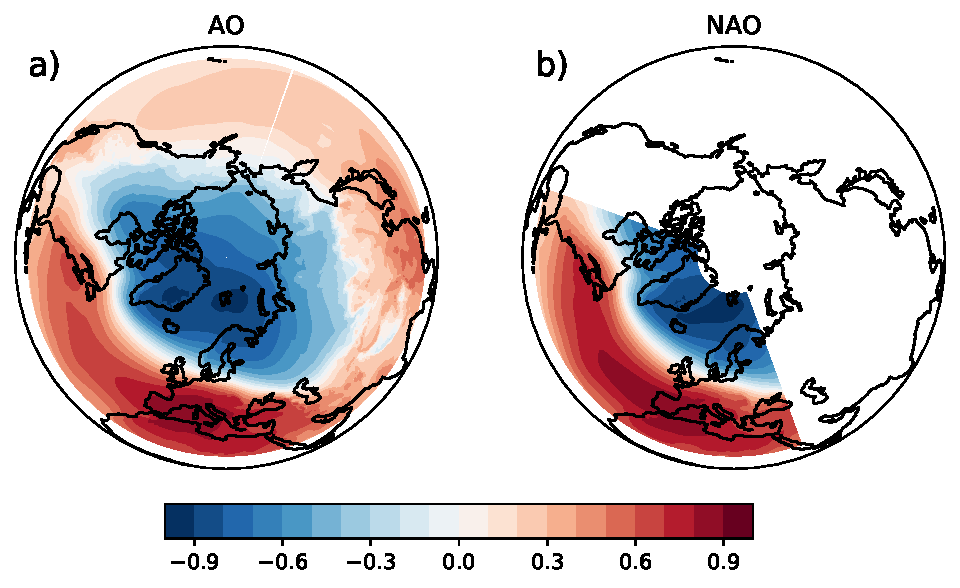
\includegraphics[width=\textwidth]{texfiles/figs/EOF_AO_NAO.pdf}
    \caption{The spatial correlation of the leading EOF of 1000hPa geopotential height (a) representing the \acrshort{ao}. (b)  spatial correlation of the leading \acrshort{eof}  of SLP anomalies over the Atlantic sector, 20\degree-80\degree N, 90\degree W-40\degree, representing the \acrshort{nao}.}
    \label{fig:EOF_NAO_AO}
\end{figure}
The \acrshort{eawm} is also influenced by large scale climatic factors, in particular previous studies have shown that the \acrfull{ao} can have a significant impact on the \acrshort{eawm} \parencite{wu2002winter,park2011relationship}. Most interesting in this context is the out-of-phase correlation between winter \acrshort{ao} and dust storm frequency reported by several recent studies \parencite{gong2006east,mao2011influence,liu2018influence}. 
The \acrshort{ao} is defined as the leading \acrfull{eof} of the 1000hPa geopotential height poleward of 20 \degree N \parencite{thompson1998arctic}. 
In its structure, it resembles the \acrfull{nao} except being more zonally symmetric as shown in \Cref{fig:EOF_NAO_AO}. 
A positive phase of the winter \acrshort{ao} is associated with positive winter \acrfull{sat} anomalies over high latitude Eurasia, with negative \acrshort{sat} anomalies over Greenland. 
Partly due to the colder temperatures a negative winter AO usually results in a stronger \acrshort{eawm} and a strengthened \acrshort{sh}.  
Cold events are also found to be more frequent over East Asia during negative AO conditions \parencite{he2017impact}.
\textcite{wu2002winter} examined how the \acrshort{ao} influence the \acrshort{eawm} and found that the AO directly influences  \acrshort{sat}, \acrshort{mslp} and the mid-level \acrshort{eat} rather than directly impacting the \acrshort{sh}.

\begin{figure}[htpb]
    \centering
    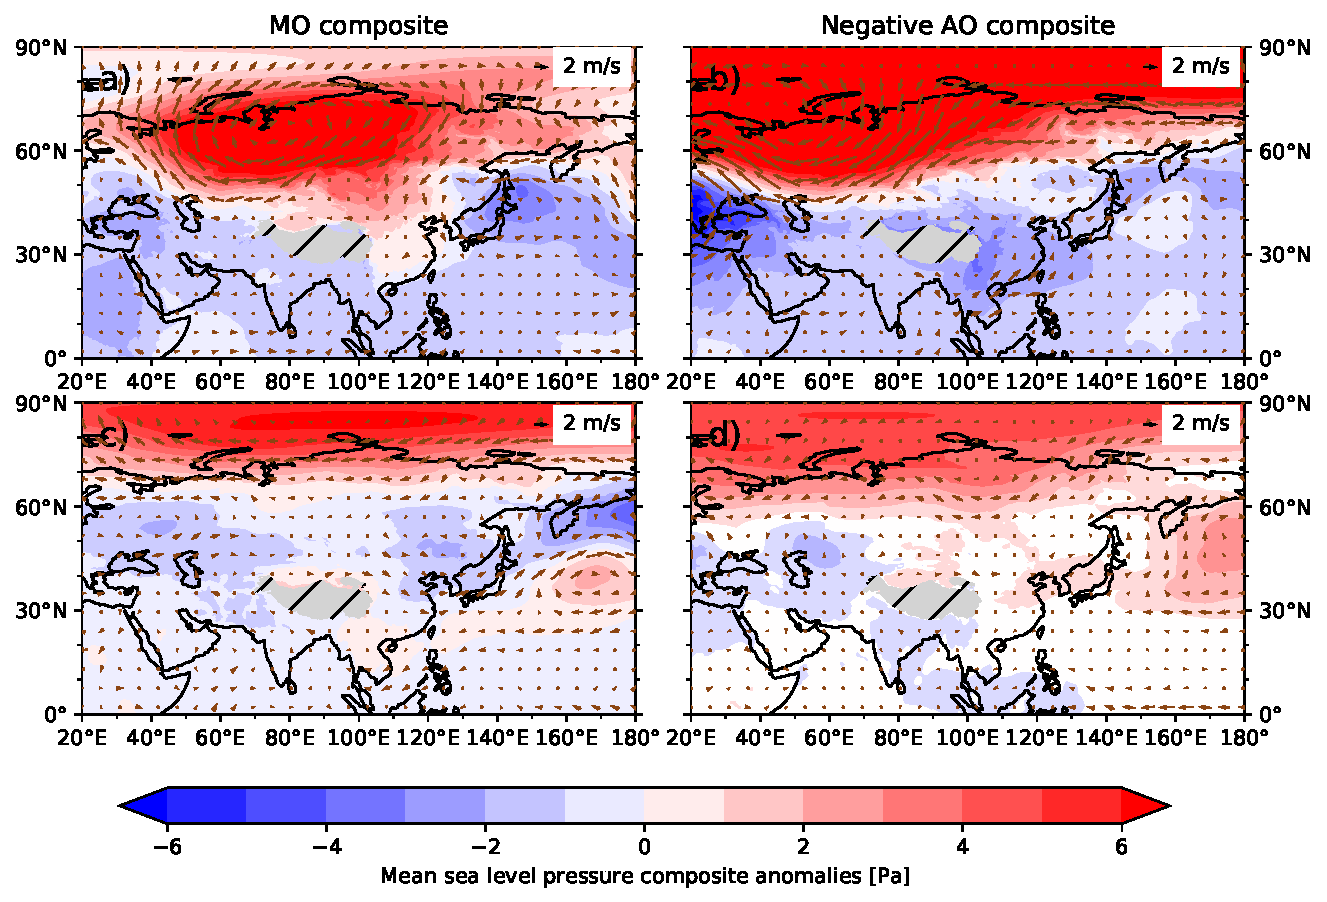
\includegraphics[width=\textwidth]{texfiles/figs/winter_MO_AO_composite.pdf}
    \caption{Circulation composite anomalies of 850hPa winds (vectors, unit: m/s) and mean sea level pressure for strong (colored, unit: Pa) - weak winter monsoon years and negative - positive winter AO. (a) and (b) is the \acrshort{djf} anomalies and (c) - (d) is MAM anomalies in the following spring}
    \label{fig:mo_ao_composite}
\end{figure}
 

\Cref{fig:mo_ao_composite} shows winter and spring composite anomalies  of the \acrshort{eawm} intensity index (MO-index), defined as the difference in \acrfull{mslp} between two grid points of (105\degree E, 52.5°N) near Irkutsk and (145\degree E, 43.75\degree N) near Nemuro and the \acrshort{ao}. 
In the negative \acrshort{ao} winters there are large positive \acrshort{mslp} anomalies over the arctic region with anti-cyclonic circulation anomalies around Barent Sea, while in the strong \acrshort{eawm} years the positive pressure anomalies are primarily confined to central Siberia. In the 500hPa level composite shown in \Cref{fig:mo_ao_composite_500hPa}; the negative geopotential anomalies has a centre over eastern China and the Korean peninsula during strong \acrshort{eawm} years, compared to the negative \acrshort{ao} years where centre is located over the Mongolian plateau. More importantly the negative geopotential anomalies persist into the following spring  (\Cref{fig:mo_ao_composite_500hPa}d). \textcite{liu2018influence} proposed that during negative \acrshort{ao} winters, northeasterly wind anomalies brings cold arctic air into central Siberia cooling the land surface. Further the anomalous cold surface conditions initiate positive snow-albedo and cloud albedo feedbacks that lasts into the following spring.  

\begin{figure}[htbp]
    \centering
    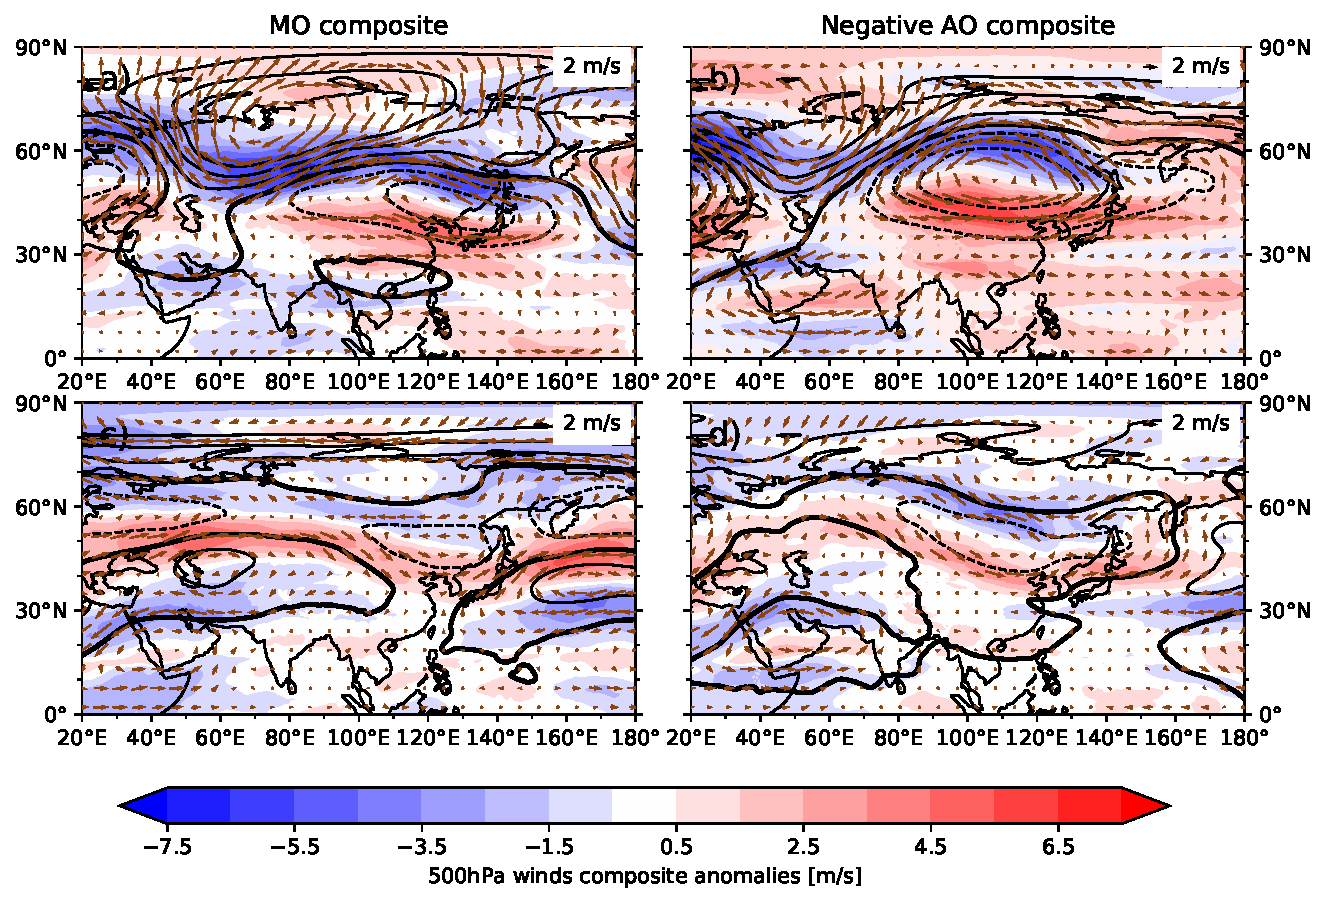
\includegraphics[width=\textwidth]{texfiles/figs/winter_MO_AO_composite_500h.pdf}
    \caption{Circulation composite anomalies of 500hPa winds strength (colored, unit m/s), wind direction (vectors, unit m/s) and geopotential height (contours, unit dam, distance between contours 2 dam) for strong - weak winter monsoon years and negative - positive winter AO. (a) and (b) is the DJF anomalies and (c) - (d) is MAM anomalies in the following spring. Data from ERA5.}
    \label{fig:mo_ao_composite_500hPa}
\end{figure}



% it has been known that there are three major motions of wind‐blown sand particles, i.e., creep, saltation, and suspension

% Except for dust storms in which the suspension motion is dominant, saltation plays a key role in the wind erosion process

%And, southwest of the plateau, the bottom of the Old Tarim Basin and Old Junggar Basin had also lifted to 1000 m elevation but still remained lower than the surrounding topography. The modern Tarim Basin and Junggar Basin are surrounded by the Altaj Mountains in the north, Tainshan Mountains in between, Tibetan Plateau in the south, Pumir Plateau in the west, and Mongolian Plateau and Kunlun Mountains in the east

%It is suggested that the source region in East Asia consists of two parts or systems: (i) the Mongolian Plateau dust source system, including deserts and gobi-deserts on the Mongolian Plateau and its southern extension—the Ordos Plateau and Alxa Plateau; and (ii) the Tarim Basin dust source system, including deserts and gobi-deserts in the Tarim Basin, Junggar Basin, and eastern vicinity.

%classified dust storms in East Asia into four types, among which the S (stationary) type and M (moving) type are basic ones. 80\% of their S type dust storms occurred over the Taklimakan Desert and vicinity, while 70\% of the M type originated over the gobi area and desert area of 90–105°E, i.e., the Mongolian Plateau and its southern extension.


%Gravel covering the gobi surface can effect the dust emission both positively and negatively: gravel half-buried in sand (soil) surfaces decreases the effective wind shear force on the soil surface, resulting in stress partitioning (Nickling and Gillies, 2003), and a complete stony armor strongly depresses the aeolian motion of particles (Yi et al., 2002). 

%precipitation is rare in the gobi area, less than 50 mm yr−1 (Zhao, 1994), and is limited to the summer season so that the gobi surface becomes extremely dry in spring when the strong wind behind a cold front periodically blows through East Asia and is enhanced over the vast and flat gobi surface. As the surface wind speed often reaches 24–30 m s−1, or even higher, on the south Mongolian Plateau (Qian et al., 1997), strong dust storms occur in spite of the gravel armoring and the below 0°C air temperature. 

%Thousands of kilometers from the oceans and high above the sea level, the Mongolian climate is extremely dry, continental and cold.

%  It is also normal in Mongolia that the annual precipitation varies greatly from year to year. For example, the precipitation in Sainshand (44°52′N, 110°09′E) was 83 mm yr−1 in 1963 but, in the next year, it went up to 248 mm yr−1 (CMA, 1970). Such a great interannual change in precipitation means that, in drought years, severe dust storms occur even in the north mountain area. At the end of winter season, the south Siberian anti-cyclone named the ‘Siberian High’ becomes unstable and, in the following spring months, breaks down several times so that a succession of frontal systems traverses the country from northwest to southeast, resulting in strong surface wind, which is further strengthened over the vast and flat gobi surface. 

%In the Mongolian Plateau system and downwind vicinity, from northwest to southeast, the surface soil texture shows a coarse-to-fine trend: gobi gravel becomes desert sand, followed by silt and clay of the Loess Plateau. 
